In order to show an improvement on existing predictive simulation systems for CHD corrective surgeries, we want to demonstrate that our blood vessel model based on thin shell elements is
\begin{enumerate}
\item physically accurate,
\item converges to expected results with a low amount of elements,
\item is able to simulate low-level surgical procedures universally.
\end{enumerate}
A quantitative validation by means of a comparision to real pre- and post-surgery image data is impossible at present. This is mainly due to ethical issues that arise during image data acquirement of infants, i.e. necessary heart rate lowering medications or exposure to radiation. There is no such data available that is obtained shortly after surgeries in infants where the growth of the patient would not interfere comparison. However, qualitative comparisons to a real image data set acquired months after a surgical intervention and to an elastic tube manipulated by hand, which confirm a principal suitability of predictive simulations for surgery planning, can be found in \cite{Li2009}.

We close this section with a discussion about the limitations and constraints of our approach which have great impact on the mesh generation prior to simulation.

\subsection{Accuracy}

Figure \ref{fig-deformations} shows bending and twisting of an elastic tube manipulated by hand compared to the simulation results of \cite{Li2009} and our method. These kinds of blood vessel deformations are likely to occur during surgery. Our results are close to the real deformations as expected due to the physically based formulation of thin shell elements.

\subsection{Convergence}

It is important to minimize the number of shell elements to reduce computation time. This is the key factor to enable an interactive simulation system that is accepted by surgeons to simulate multiple surgical approaches in succession. The bending of thin shell elements allows to reduce their number by still representing the tubular structure of blood vessels while maintaining their physical behavior appropriately. Figure \ref{fig-convergence} shows simulation results of a strongly deformed tube represented by different numbers of thin shell elements. With only eight vertices along the circumference of the tube the simulation result is comparable to a simulation result with high element count. We map a fine polygonal mesh to the coarse shell element meshes to visualize their bending detail and therefore get comparable results that correlates with the true shape of the simulated tube.

\subsection{Low-level surgical procedures}

\begin{figure}[tbh]
  \centering
  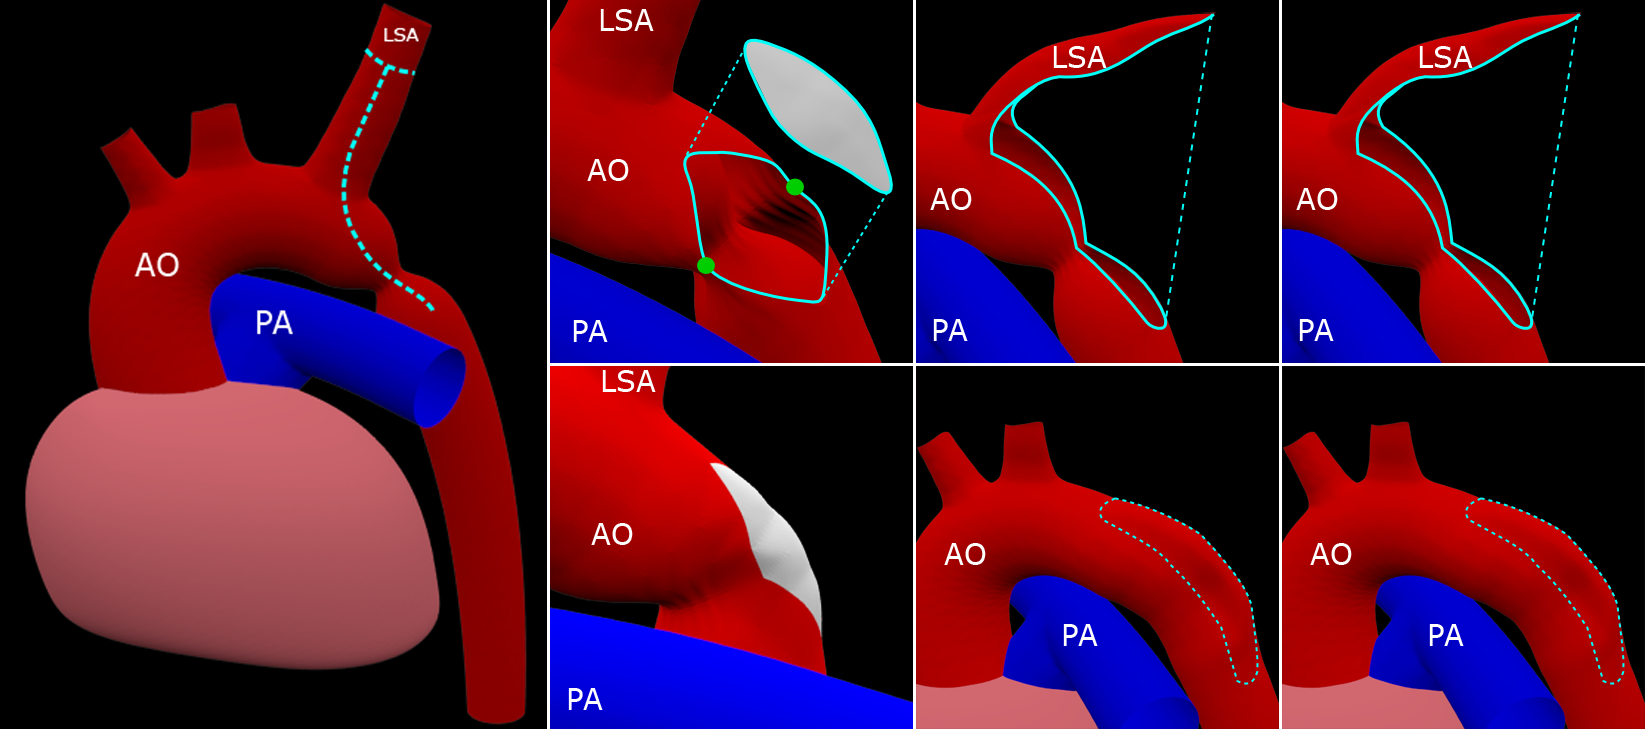
\includegraphics[width=\columnwidth]{img/surgery.png}
  \caption{Bla.}
\end{figure}

TODO: Use the remaining space we have in the paper. We should consider to shorten other sections.

\subsection{Limitations and Constraints}

%Example with 3 diff. surgical procedures
%Parameters
%Limitations (getting image data, meshes, dynamic remeshing, same number of nodes)
